82. $f(x)=\cfrac{2-|x+3|}{x}=\begin{cases} \cfrac{2+x+3}{x},\ x\leqslant-3,\\
\cfrac{2-x-3}{x},\ x>-3.\end{cases}=\begin{cases} 1+\cfrac{5}{x},\ x\leqslant-3,\\
-1-\cfrac{1}{x},\ x>-3.\end{cases}$\\
а) $$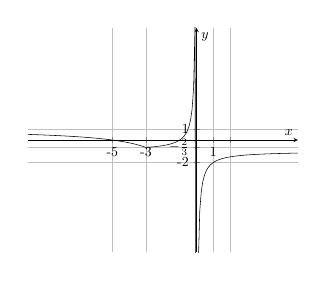
\begin{tikzpicture}[scale=0.5]
\begin{axis}[
    axis lines = middle,
    grid=major,
    legend pos={south west},
    xlabel = {$x$},
    %xlabel style={below right},
    ylabel = {$y$},
    ymin=-10,
    ymax=10,
    xmin=-10,
    xmax=6,
    xtick={-5, -3,  1, 2},
    xticklabels={-5, -3, 1, $ $},
    ytick={-2,-0.66, 1},
    yticklabels={-2,$-\frac{2}{3}$, 1},
                  ]
	\addplot[domain=-10:-3, samples=100, color=black] {1+5/x};
    \addplot[domain=-2.99:6, samples=100, color=black] {-1-1/x};
        %\addplot[domain=2.01:6, samples=100, color=black] {2/(2-x)};
   % \addplot[domain=-3:3, samples=100, color=black] {-x};
     %\addlegendentry{$\text{Рис. 1}$};
\end{axis}
%\draw (5.71,2.59) circle (2pt);
%\draw (3.45,0.75) circle (2pt);
%\draw (3.45,2.55) circle (2pt);
\end{tikzpicture}$$
б) При $x<0$ график функции находится выше уровня $y=-\cfrac{3}{2}.$ Если $-1-\cfrac{1}{x}=-\cfrac{3}{2},$ то $\cfrac{1}{x}=\cfrac{1}{2},\ x=2.$ Значит, $f(x)\geqslant -\cfrac{3}{2}$ при $x\in(-\infty;0)\cup[2;+\infty).$\\
в) Горизонтальными асимптотами являются $y=-1$ и $y=1,$ исходя из этого найдём количество решений: при $a\in\left[-1;-\cfrac{2}{3}
ight):0,$ при $a\in(-\infty;-1)\cup\left\{-\cfrac{2}{3}
ight\}\cup[1;+\infty):1,$ при $a\in\left(-\cfrac{2}{3};1
ight):2.$\\
